\documentclass[UTF8,zihao=-4]{ctexart}
\usepackage[a4paper,margin=2.35cm]{geometry}
\usepackage{amsmath,amssymb}
\usepackage{booktabs}
\usepackage{graphicx}
\usepackage{float}
\usepackage{placeins}
\usepackage{array}
\usepackage{caption}
\usepackage{subcaption}
\usepackage{hyperref}
\usepackage{xcolor}
\hypersetup{colorlinks=true,linkcolor=black,citecolor=black,urlcolor=blue}
\setlength{\parindent}{2em}
\setlength{\parskip}{0.25em}
\renewcommand{\arraystretch}{1.16}
\captionsetup{font=small,labelfont=bf}

\title{\heiti 近五年美国股票市场结构动态变化分析\\
\large 基于滚动相关距离、MDS、聚类与简单预测的实证研究}
\author{数据挖掘课程项目：MarketManifold}
\date{2026年6月}

\begin{document}
\maketitle

\begin{abstract}
本文使用本地历史行情压缩包中的真实美国股票日频数据，构建覆盖信息技术、金融、医疗、能源、消费、工业、通信服务、公用事业、材料和房地产等行业的固定大市值股票池，研究近五年股票收益率结构的动态变化。方法上，本文在90个交易日滚动窗口中计算股票收益相关矩阵，将相关系数转换为相关距离，并使用多维尺度分析(MDS)得到二维市场结构图；同时以PCA作为对照降维方法，以凝聚层次聚类和KMeans观察数据驱动分组，并用Procrustes正交对齐降低相邻窗口坐标的旋转和翻转。结果显示，平均相关性、等权市场年化波动率和第一主成分解释率高度同步：三者两两相关系数分别达到0.959、0.993和0.978。最高波动窗口结束于2022-08-30，市场波动率为0.261，平均相关性为0.510；最高相关窗口结束于2022-12-22，平均相关性为0.543，第一主成分解释率为0.564。最新窗口结束于2026-06-15，平均相关性下降至0.105，二维平均距离上升至1.159，显示结构较高相关时期更加分散。简单预测实验中，LinearRegression和RandomForestRegressor在时间顺序测试集上均优于naive baseline，但该结果仅表明窗口指标存在短期自相关和线性可预测成分，不构成投资建议。
\end{abstract}

\noindent\textbf{关键词：} 市场结构；相关距离；多维尺度分析；滚动窗口；聚类；Procrustes对齐；股票收益率

\section{引言}
股票市场并不是一组相互独立的价格序列。宏观冲击、流动性变化、行业景气和投资者风险偏好会使股票收益在不同阶段呈现不同程度的共同运动。当市场压力上升时，个股之间的相关性常常同步提高，低维结构中不同股票可能向中心靠拢；而在较平稳阶段，行业基本面和公司特质可能重新主导横截面差异。对这种结构变化进行量化，有助于理解“市场作为整体”和“股票作为个体”之间的动态关系。

本文的课程目标不是构建交易策略，而是完成一个可复现的数据挖掘实验：从真实历史数据中抽取固定股票池，清洗价格序列，构建收益率矩阵，在滚动窗口中分析相关结构、低维嵌入、聚类稳定性和简单预测能力。与只画指数时间序列不同，本文关注每个窗口内股票之间的相对位置、聚集与分离，并把行业标签与数据驱动聚类进行比较。所有结论均基于项目生成的CSV结果表，本文不使用模拟数据作为正式实验结果。

需要说明的是，原始压缩包呈现Stooq-style日频文本数据格式，包括按市场和股票分层的目录结构、以\texttt{aapl.us.txt}为代表的文件名，以及ticker、period、date、open、high、low、close、volume等行情字段，但压缩包中没有独立说明文件。因此本文将数据来源写作“Stooq-style，未独立确认”。价格字段仅包含\texttt{close}，没有明确的adjusted close字段，也没有文件说明证明其为复权价格；因此本文记录复权状态为\texttt{unknown}，并避免把\texttt{close}称为已复权价格。

\section{研究问题与数据}
\subsection{研究问题}
本文围绕六个问题展开。第一，近五年美国大市值股票收益率相关结构是否稳定。第二，股票在滚动窗口二维空间中如何聚集、分离和迁移。第三，市场平均相关性、整体波动率和共同因子强度是否同步变化。第四，高波动时期市场结构是否更集中。第五，行业标签与数据驱动聚类之间在何种程度上一致。第六，窗口级结构指标是否能用于预测下一窗口的市场波动率。

\subsection{数据集概况}
原始ZIP包含12404个成员，其中12391个为\texttt{.txt}文本文件。项目从中匹配46只目标股票，最终46只全部保留。实验实际区间为2021-06-22至2026-06-22，共1255个共同有效交易日。表\ref{tab:data-overview}给出数据集概况。

\begin{table}[H]
\centering
\caption{数据集概况}
\label{tab:data-overview}
\small
\begin{tabular}{p{0.28\textwidth}p{0.62\textwidth}}
\toprule
项目 & 数值或说明 \\
\midrule
数据格式判断 & Stooq-style daily US text archive, not independently confirmed \\
组织方式 & 每个标的一个文本文件 \\
检测字段 & ticker, period, date, time, open, high, low, close, volume, open interest \\
日期格式 & YYYYMMDD \\
价格字段 & close \\
价格复权状态 & unknown \\
原始最早日期 & 1962-01-02 \\
原始最晚日期 & 2026-06-22 \\
实验起始日期 & 2021-06-22 \\
实验结束日期 & 2026-06-22 \\
请求股票数 & 46 \\
匹配股票数 & 46 \\
最终保留股票数 & 46 \\
最终交易日数 & 1255 \\
最终长表行数 & 57730 \\
行业数量 & 11 \\
无效价格数 & 0 \\
异常收益数($|\log return|>0.5$) & 0 \\
\bottomrule
\end{tabular}
\end{table}

\subsection{参数设置}
表\ref{tab:params}列出主要实验参数。滚动窗口采用90个交易日，步长为10个交易日，共形成117个窗口。聚类数固定为6，以便不同窗口之间可以比较标签稳定性。窗口内在股票维度进行标准化，避免高波动股票在距离计算和PCA中特别主导结构。

\begin{table}[H]
\centering
\caption{主要实验参数}
\label{tab:params}
\small
\begin{tabular}{ll}
\toprule
参数 & 设定 \\
\midrule
滚动窗口长度 & 90个交易日 \\
滚动步长 & 10个交易日 \\
窗口数量 & 117 \\
聚类数量 & 6 \\
最低覆盖率 & 90\% \\
短缺口填充 & 最多向前填充2个交易日 \\
收益率处理 & 对数收益率，0.5\%和99.5\%分位winsorize \\
主降维方法 & 基于相关距离矩阵的MDS \\
主聚类方法 & AgglomerativeClustering, average linkage \\
对照方法 & PCA + KMeans \\
随机种子 & 42 \\
\bottomrule
\end{tabular}
\end{table}

\section{方法}
\subsection{对数收益率}
设股票$i$在交易日$t$的价格为$P_{i,t}$。本文使用对数收益率
\begin{equation}
r_{i,t}=\log P_{i,t}-\log P_{i,t-1}.
\end{equation}
对数收益率便于时间加总，也能在小幅收益情况下近似普通收益率。清洗后价格矩阵使用共同有效交易日构建，收益率矩阵记为$R\in\mathbb{R}^{T\times N}$，其中$T$为窗口内交易日数，$N=46$为股票数。

\subsection{相关距离}
对每个滚动窗口，计算股票收益相关系数矩阵$\rho_{ij}$。为了把相关性转换为满足直观几何解释的距离，本文采用Mantegna提出的相关距离形式\cite{Mantegna1999}：
\begin{equation}
d(i,j)=\sqrt{2(1-\rho_{ij})}.
\end{equation}
当两只股票完全正相关时，距离为0；当相关性下降时，距离增大。由于相关系数被限制在$[-1,1]$，该距离非负，且在完全负相关时达到2。

\subsection{MDS二维嵌入}
多维尺度分析(MDS)试图寻找二维坐标$z_i\in\mathbb{R}^2$，使二维欧氏距离尽量接近输入距离$d(i,j)$。经典和度量MDS均可理解为最小化应力函数\cite{Torgerson1952,Kruskal1964}：
\begin{equation}
\min_{z_1,\ldots,z_N}\sum_{i<j}\left(\lVert z_i-z_j\rVert_2-d(i,j)\right)^2.
\end{equation}
本文使用MDS作为主方法，是因为它直接作用于相关距离矩阵，能够把股票间的相对相关结构投影到二维图中。二维坐标只表示窗口内相对结构，不应解释为固定经济坐标轴。

\subsection{PCA对照与共同因子强度}
PCA对照方法将窗口内每只股票的标准化收益序列视为特征向量，寻找最大方差方向。设窗口标准化收益矩阵的协方差矩阵特征值为$\lambda_1\geq \lambda_2\geq \cdots \geq \lambda_N$，则第一主成分解释率定义为
\begin{equation}
\mathrm{PC1Ratio}=\frac{\lambda_1}{\sum_{k=1}^{N}\lambda_k}.
\end{equation}
该指标可被视为共同因子强度的经验度量。当大多数股票共同运动增强时，第一主成分往往解释更多横截面收益方差\cite{Jolliffe2002}。

\subsection{Procrustes动态对齐}
不同窗口独立MDS会产生任意旋转、镜像和平移，直接制作动画会出现坐标轴抖动。本文使用正交Procrustes对齐\cite{Schonemann1966}。给定上一窗口已对齐坐标$X$和当前窗口原始坐标$Y$，先分别中心化：
\begin{equation}
X_c=X-\bar{X},\quad Y_c=Y-\bar{Y}.
\end{equation}
然后求正交矩阵$Q$：
\begin{equation}
Q^*=\arg\min_{Q^\top Q=I}\lVert Y_cQ-X_c\rVert_F^2.
\end{equation}
最终对齐坐标为
\begin{equation}
\tilde{Y}=(Y-\bar{Y})Q^*+\bar{X}.
\end{equation}
这里仅允许平移、旋转和镜像，不引入缩放。因此对齐前后的两两距离应保持不变。修复后的诊断表显示，所有窗口的对齐前后平均两两距离比位于$[1.000,1.000]$，最后窗口的原始坐标范数和对齐坐标范数均为0.888。

\subsection{聚类和稳定性指标}
主方法在相关距离矩阵上使用凝聚层次聚类，聚类数设为6；对照方法在PCA特征空间中使用KMeans。聚类编号只是算法标签，不能直接解释成固定行业。为了比较相邻窗口聚类稳定性，本文使用Adjusted Rand Index (ARI)\cite{HubertArabie1985}。若两组标签为$U$和$V$，ARI可写为
\begin{equation}
\mathrm{ARI}=\frac{\mathrm{RI}-\mathbb{E}[\mathrm{RI}]}{\max(\mathrm{RI})-\mathbb{E}[\mathrm{RI}]},
\end{equation}
其中RI为Rand Index。ARI接近1表示分组高度一致，接近0表示与随机分组相近。本文还计算行业标签与数据驱动聚类之间的ARI和NMI，用于衡量行业解释力。

\subsection{市场波动率和横截面指标}
设等权市场收益为
\begin{equation}
r_{m,t}=\frac{1}{N}\sum_{i=1}^{N}r_{i,t}.
\end{equation}
窗口级市场年化波动率定义为
\begin{equation}
\sigma_m=\sqrt{252}\cdot \mathrm{sd}(r_{m,t}).
\end{equation}
此外，本文记录平均相关性、中位相关性、横截面离散度、二维平均两两距离、轮廓系数、相邻窗口ARI和行业-聚类ARI等指标。

\section{结果}
\subsection{窗口指标描述统计}
表\ref{tab:metric-desc}给出117个窗口的主要指标描述统计。平均相关性均值为0.256，最大值为0.543，最小值为0.085。市场年化波动率均值为0.146，最大值为0.261。PC1解释率均值为0.305，最大值为0.564。二维平均距离的最小值出现在高度相关窗口附近，说明相关性增强时股票在二维结构中更集中。

\begin{table}[H]
\centering
\caption{窗口指标描述统计}
\label{tab:metric-desc}
\small
\begin{tabular}{lrrrr}
\toprule
指标 & 均值 & 标准差 & 最小值 & 最大值 \\
\midrule
平均相关性 & 0.256 & 0.132 & 0.085 & 0.543 \\
中位相关性 & 0.260 & 0.138 & 0.081 & 0.548 \\
市场年化波动率 & 0.146 & 0.055 & 0.078 & 0.261 \\
PC1解释率 & 0.305 & 0.121 & 0.152 & 0.564 \\
横截面离散度 & 0.015 & 0.001 & 0.012 & 0.019 \\
二维平均距离 & 1.049 & 0.096 & 0.823 & 1.166 \\
轮廓系数 & 0.109 & 0.033 & 0.054 & 0.208 \\
相邻窗口ARI & 0.741 & 0.176 & 0.350 & 1.000 \\
行业-聚类ARI & 0.163 & 0.056 & 0.045 & 0.287 \\
\bottomrule
\end{tabular}
\end{table}

\begin{figure}[H]
\centering
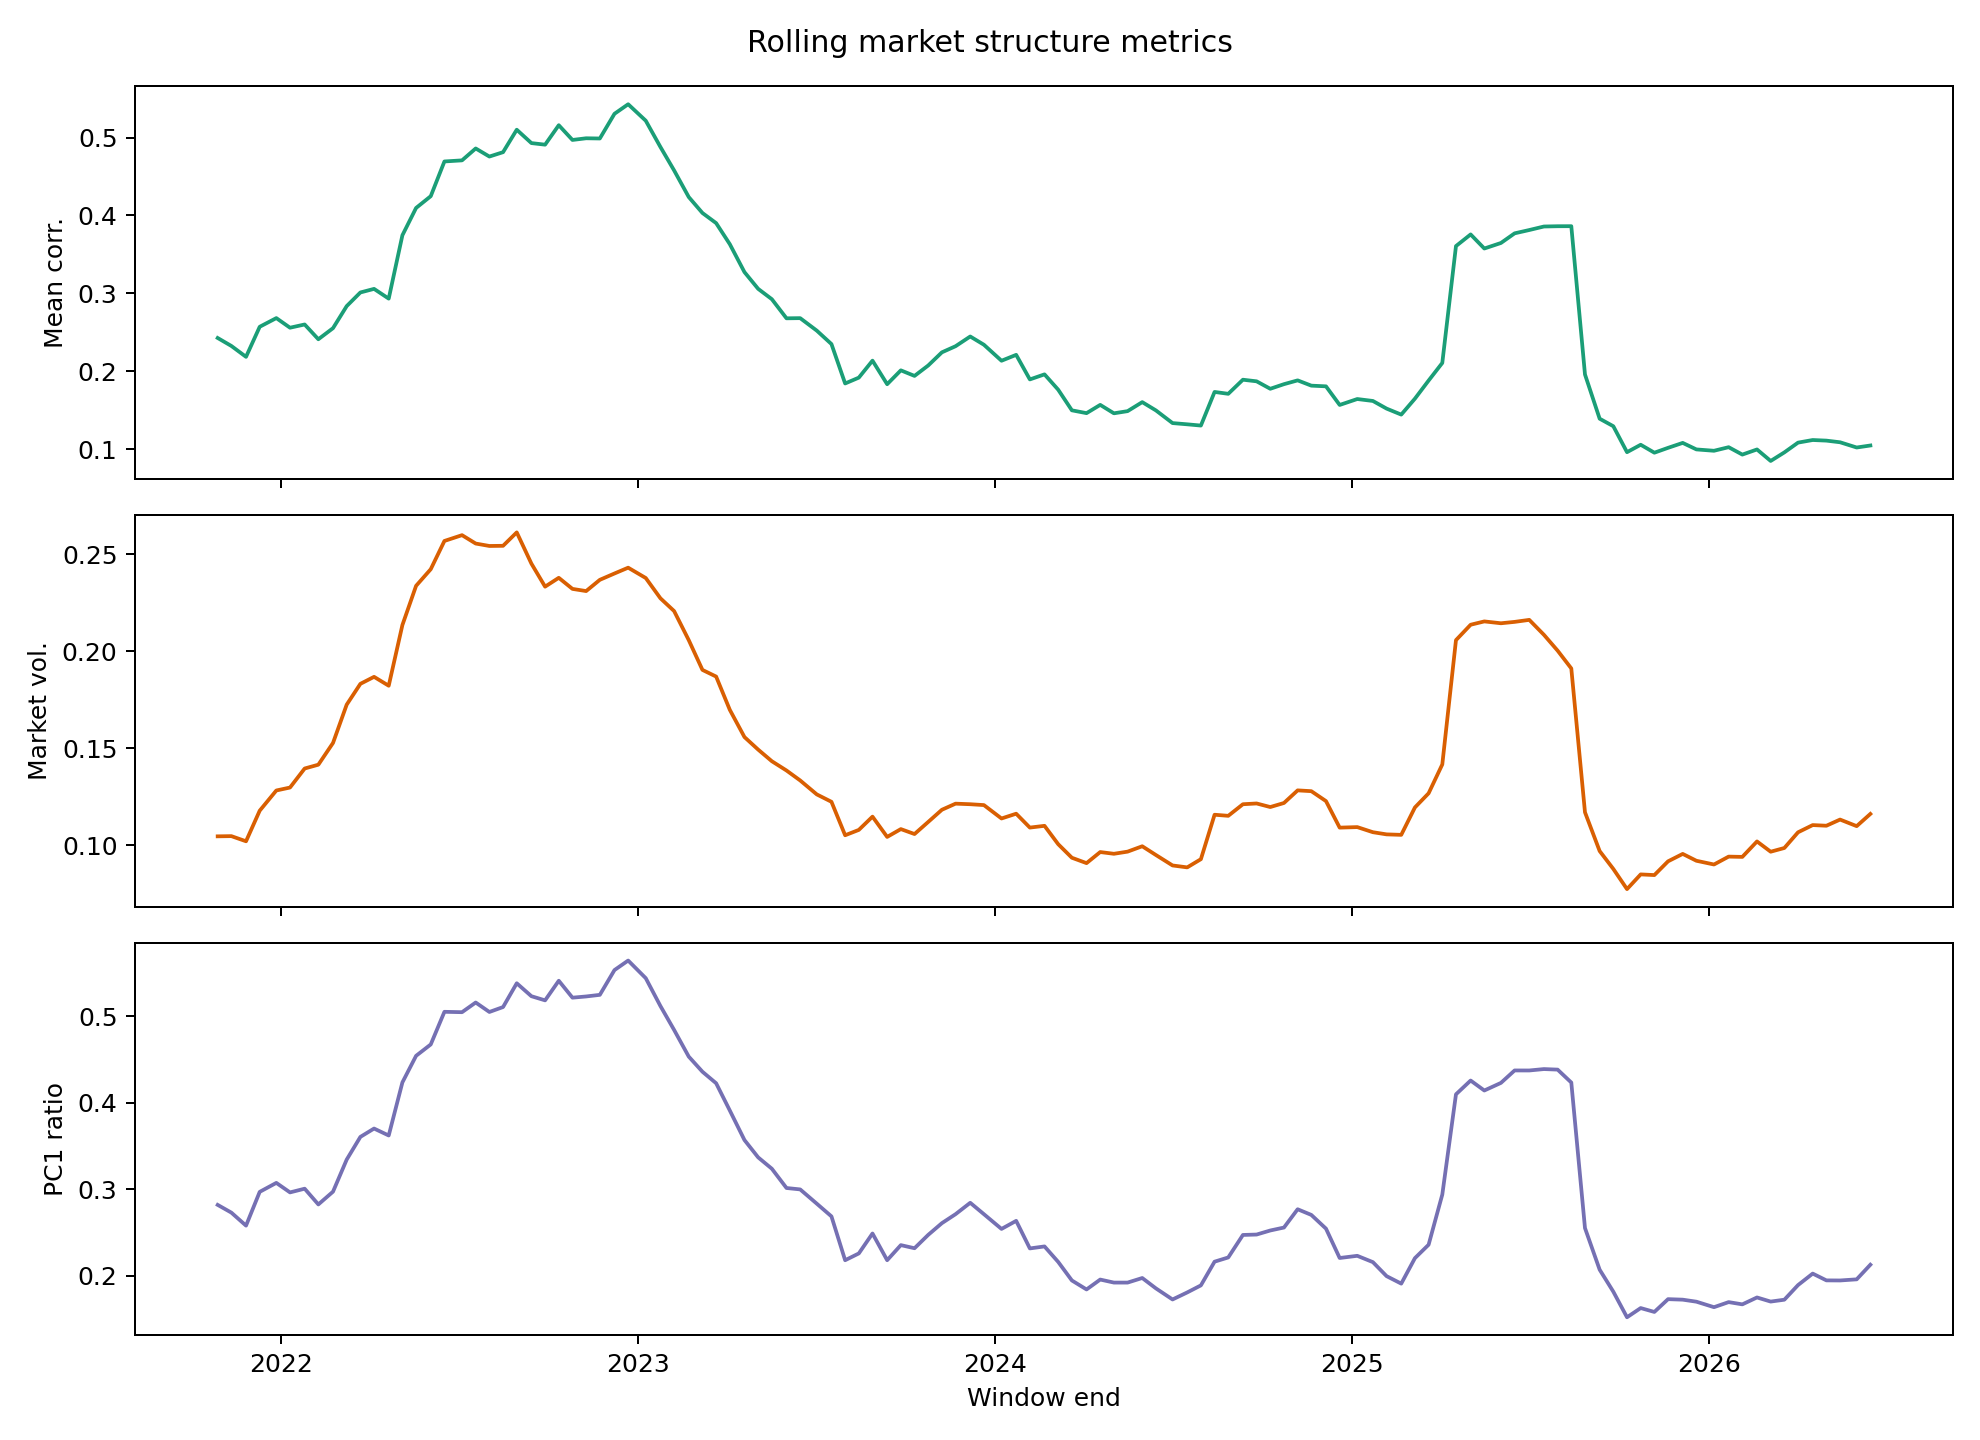
\includegraphics[width=0.92\textwidth]{../outputs/figures/market_metrics_timeseries.png}
\caption{平均相关性、市场波动率和PC1解释率的滚动变化}
\label{fig:metrics}
\end{figure}

图\ref{fig:metrics}显示，平均相关性、市场波动率和PC1解释率在样本中高度同步。三者的相关系数矩阵为：平均相关性与市场波动率0.959，平均相关性与PC1解释率0.993，市场波动率与PC1解释率0.978。这说明窗口内共同因子强度并非孤立变化，而是与整体市场波动和股票间相关性一起上升或下降。特别是在2022年中后期，三个指标同时处于高位，低维结构也表现为更小的平均两两距离。

\subsection{关键窗口比较}
表\ref{tab:key-windows}比较三个关键窗口：最高波动窗口、最高相关窗口和最新窗口。最高波动窗口结束于2022-08-30，市场波动率为0.261，平均相关性为0.510，PC1解释率为0.538。最高相关窗口结束于2022-12-22，平均相关性达到0.543，PC1解释率达到0.564，同时二维平均距离降至0.823，是样本中最集中的结构之一。最新窗口结束于2026-06-15，平均相关性为0.105，市场波动率为0.116，PC1解释率为0.213，二维平均距离为1.159，说明与2022年的集中状态相比，股票间结构更分散。

\begin{table}[H]
\centering
\caption{关键窗口指标}
\label{tab:key-windows}
\small
\begin{tabular}{lrrrrrr}
\toprule
窗口 & 结束日 & 平均相关 & 市场波动 & PC1解释率 & 轮廓系数 & 二维平均距离 \\
\midrule
最高波动 & 2022-08-30 & 0.510 & 0.261 & 0.538 & 0.197 & 0.861 \\
最高相关 & 2022-12-22 & 0.543 & 0.243 & 0.564 & 0.087 & 0.823 \\
最新窗口 & 2026-06-15 & 0.105 & 0.116 & 0.213 & 0.134 & 1.159 \\
\bottomrule
\end{tabular}
\end{table}

\begin{figure}[H]
\centering
\begin{subfigure}{0.49\textwidth}
\centering
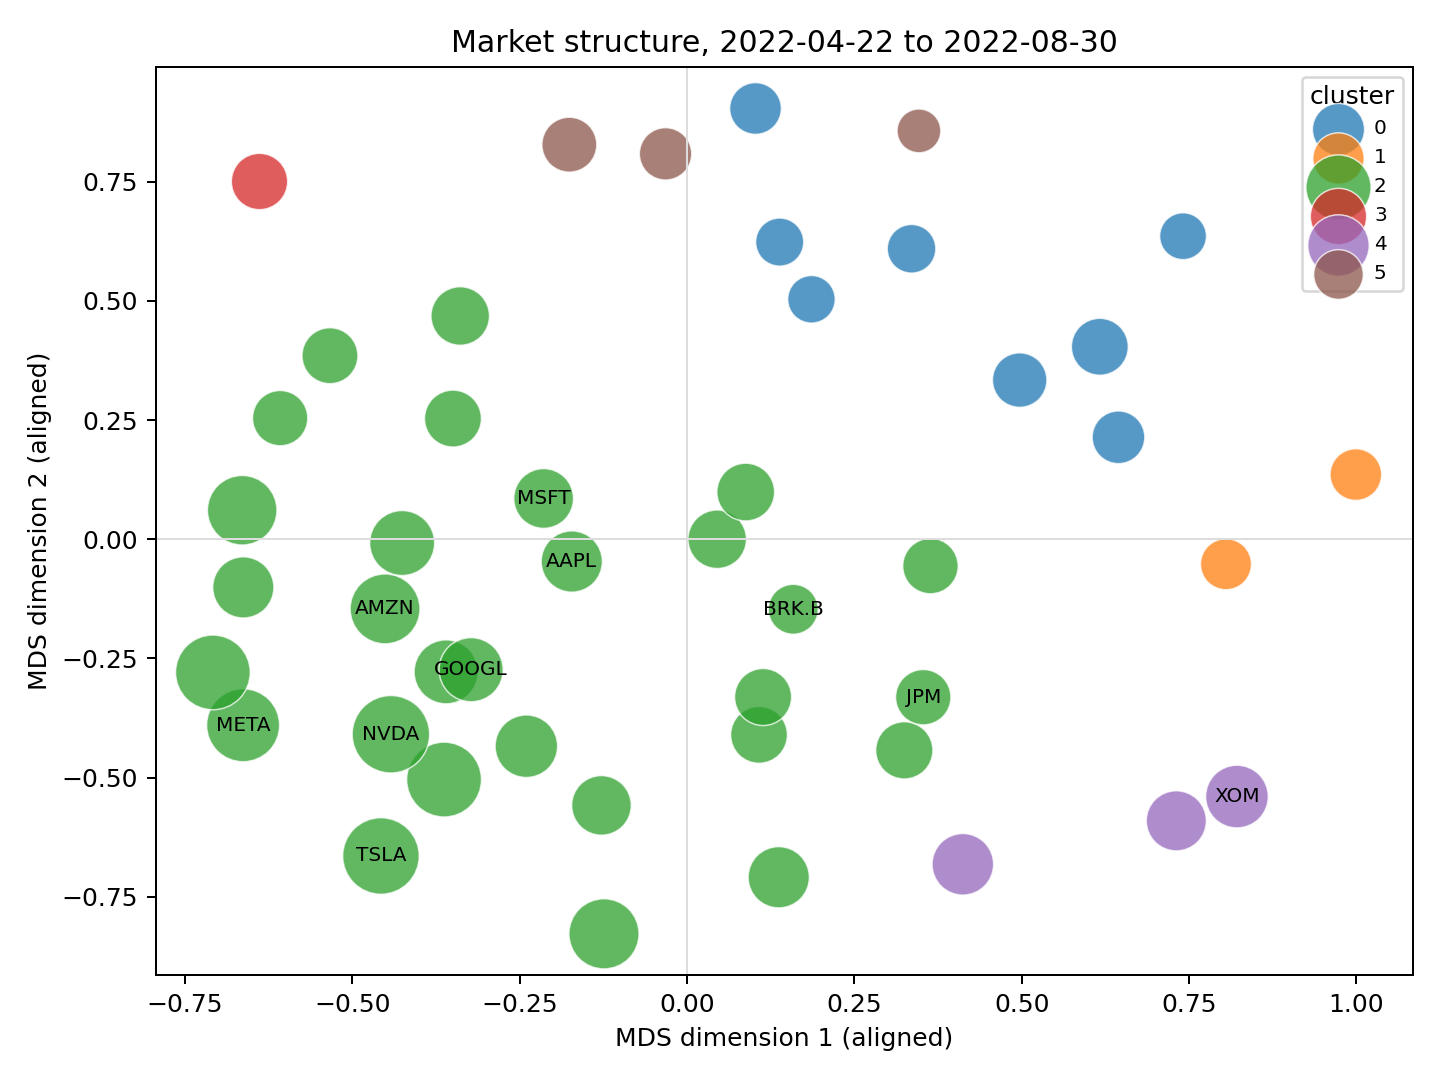
\includegraphics[width=\textwidth]{../outputs/figures/key_snapshot_1.png}
\caption{最高波动窗口}
\end{subfigure}
\begin{subfigure}{0.49\textwidth}
\centering
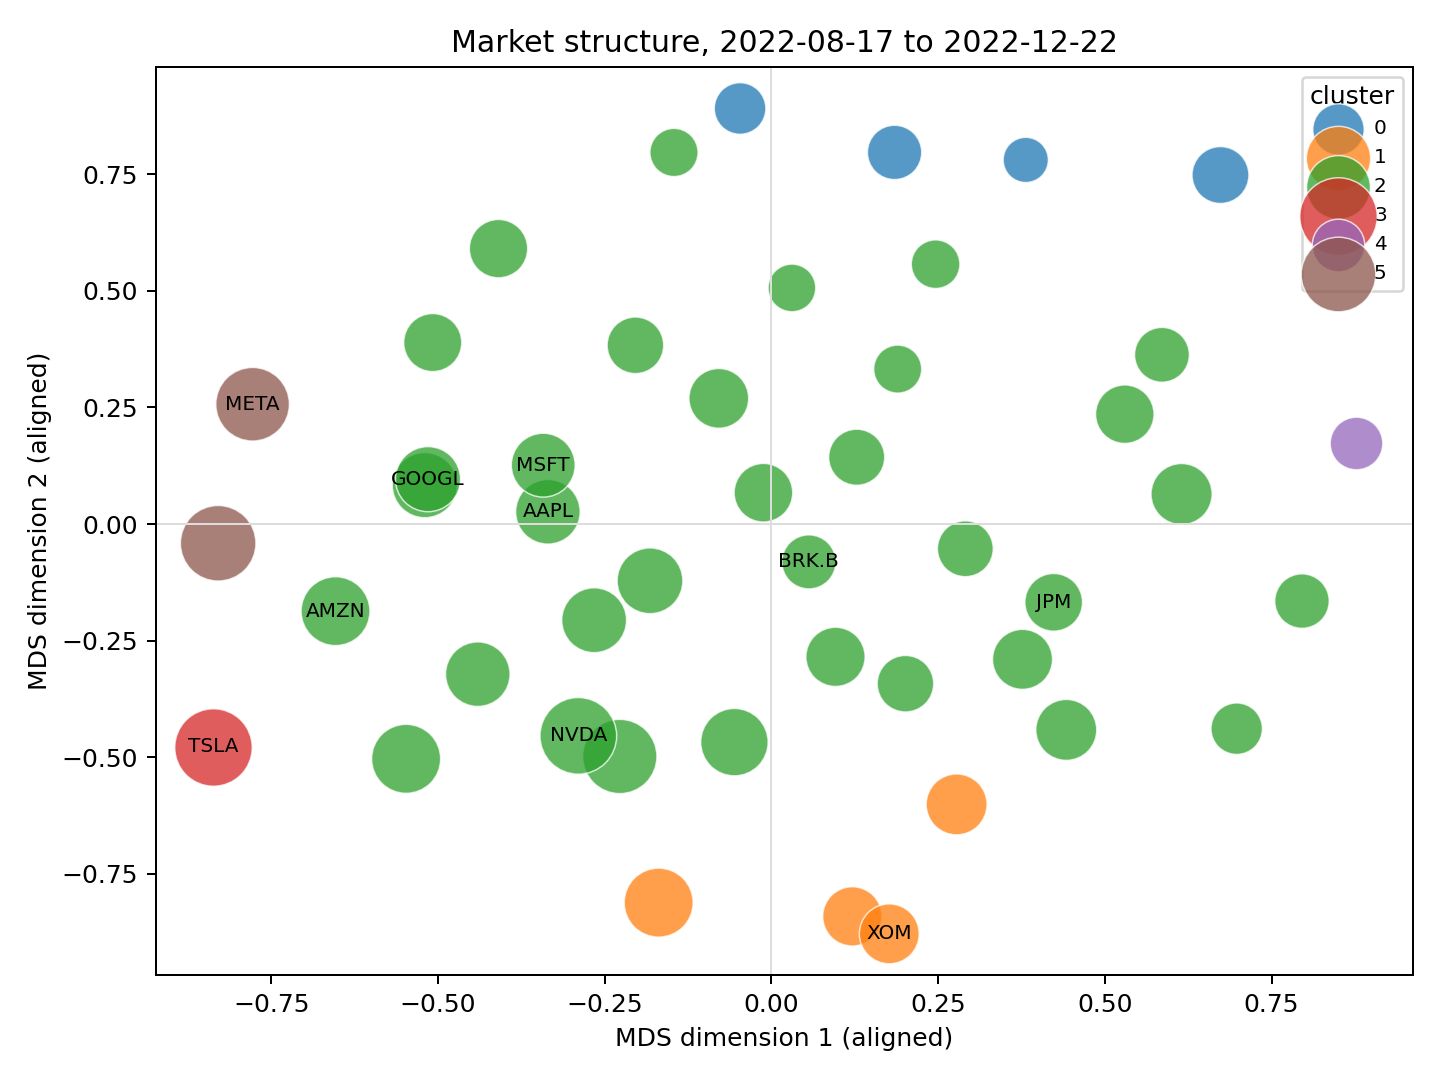
\includegraphics[width=\textwidth]{../outputs/figures/key_snapshot_2.png}
\caption{最高相关窗口}
\end{subfigure}
\vspace{0.3em}
\begin{subfigure}{0.62\textwidth}
\centering
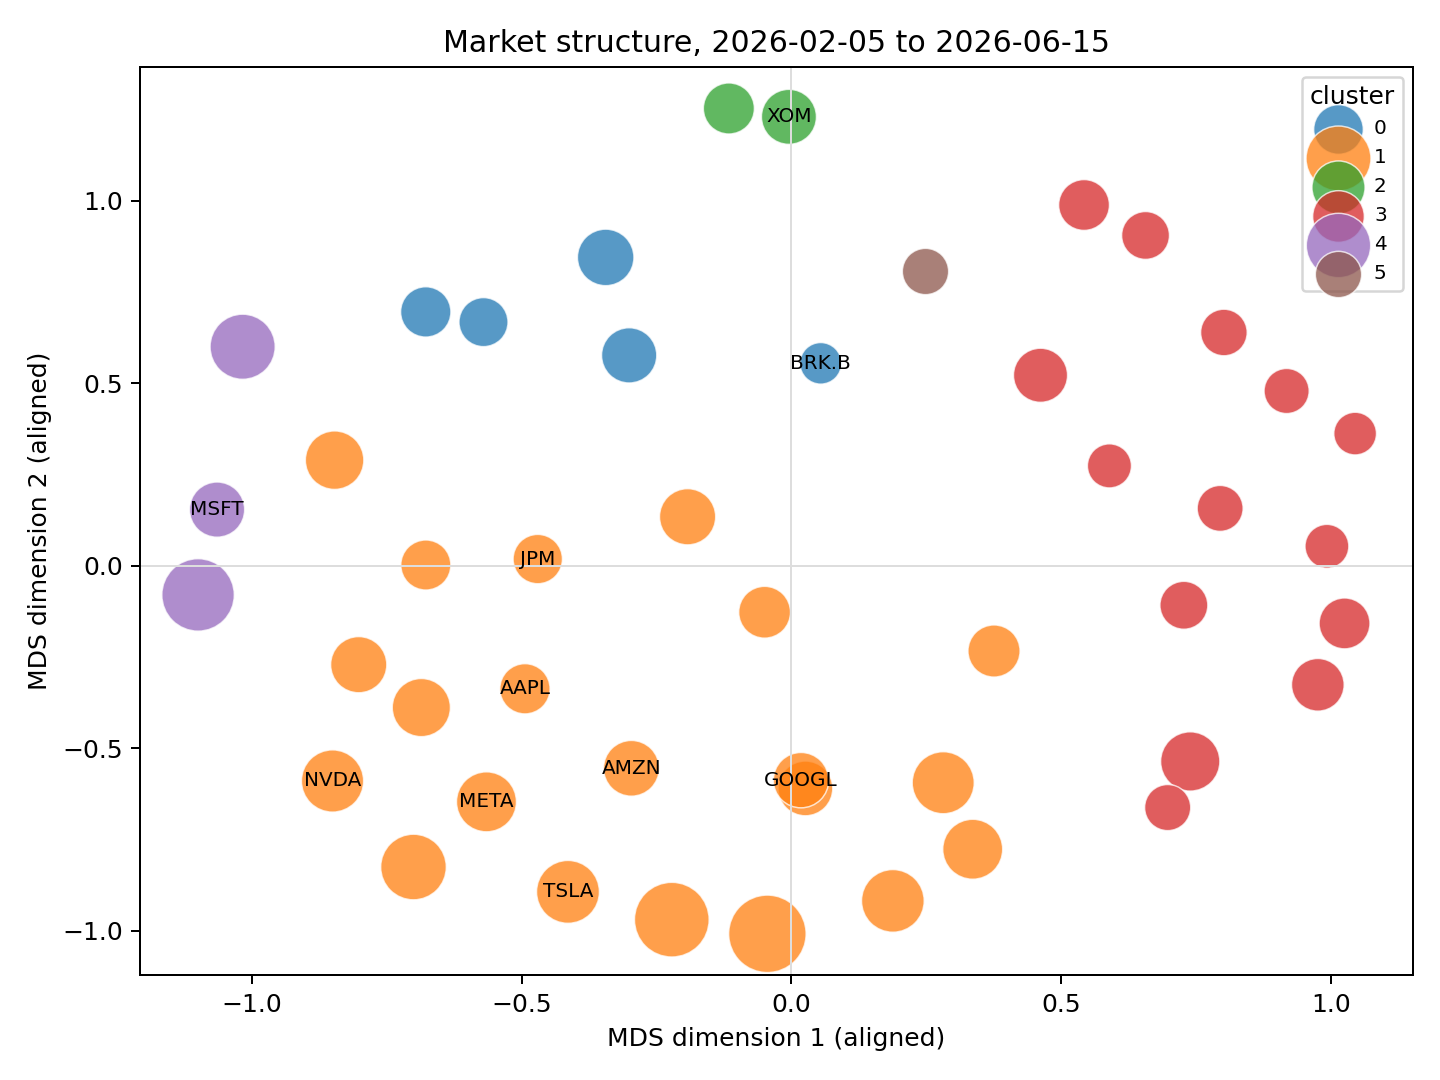
\includegraphics[width=\textwidth]{../outputs/figures/latest_market_structure.png}
\caption{最新窗口}
\end{subfigure}
\caption{三个关键窗口的市场结构快照}
\label{fig:snapshots}
\end{figure}

图\ref{fig:snapshots}中的点代表股票，颜色代表数据驱动聚类，点大小代表窗口内股票年化波动率。最高波动和最高相关窗口中，较多股票压缩到相对集中的区域，反映平均相关性和共同因子强度上升。最新窗口中，股票坐标跨度明显扩大，平均两两距离也恢复到1.159。由于MDS坐标经过正交对齐，动画中的位置迁移可用于观察相对结构变化；但坐标轴本身仍不具有固定经济含义。

\subsection{聚类稳定性和行业解释}
聚类稳定性结果见表\ref{tab:cluster-stability}。相邻窗口ARI均值为0.741，说明大多数相邻窗口的数据驱动聚类变化并不剧烈；但最小值为0.350，表明部分窗口存在明显成员重排。行业-聚类ARI均值只有0.163，NMI均值为0.461，说明行业标签对聚类具有一定解释力，但远不足以完全解释数据驱动分组。

\begin{table}[H]
\centering
\caption{聚类稳定性和行业一致性}
\label{tab:cluster-stability}
\small
\begin{tabular}{lrrrr}
\toprule
指标 & 均值 & 标准差 & 最小值 & 最大值 \\
\midrule
相邻窗口ARI & 0.741 & 0.176 & 0.350 & 1.000 \\
行业-聚类ARI & 0.163 & 0.056 & 0.045 & 0.287 \\
行业-聚类NMI & 0.461 & 0.061 & 0.328 & 0.576 \\
轮廓系数 & 0.109 & 0.033 & 0.054 & 0.208 \\
聚类数量 & 6.000 & 0.000 & 6.000 & 6.000 \\
\bottomrule
\end{tabular}
\end{table}

\begin{figure}[H]
\centering
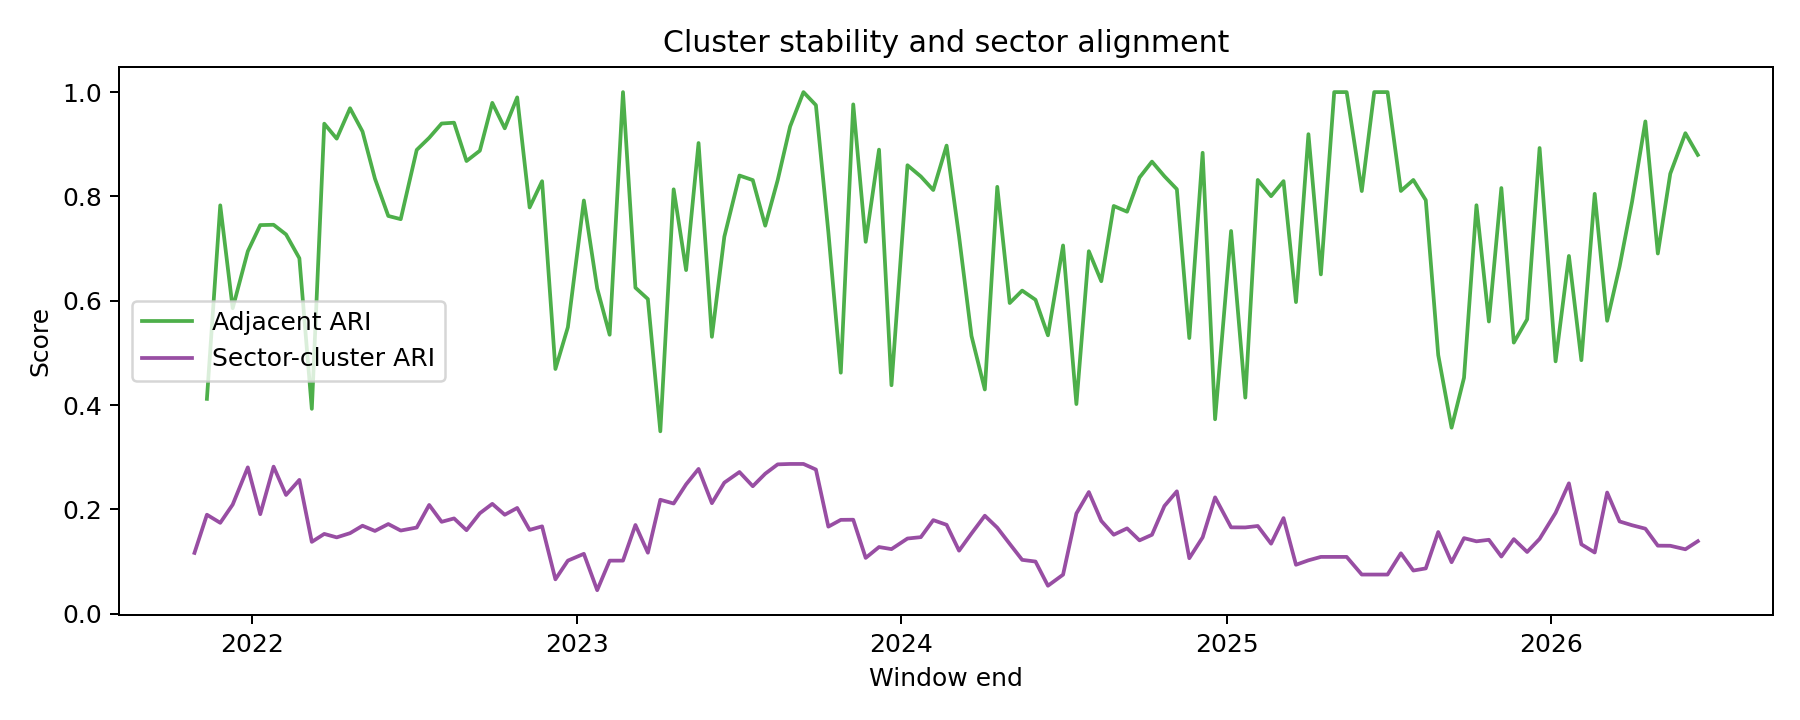
\includegraphics[width=0.86\textwidth]{../outputs/figures/cluster_stability.png}
\caption{相邻窗口聚类稳定性与行业-聚类一致性}
\label{fig:cluster-stability}
\end{figure}

从具体窗口看，最高相关窗口中一个大簇同时包含信息技术9只、金融7只、消费必需品5只、通信服务4只、可选消费4只以及其他行业股票。这种跨行业大簇说明，在高相关时期，数据驱动聚类更多反映共同市场因子，而不是简单复制行业分类。最新窗口中，信息技术、通信服务、可选消费和金融仍有交叉聚集；能源股票形成较小簇，消费必需品、医疗、公用事业也在另一簇中较集中。总体而言，行业标签在防御性行业或能源行业上有一定解释力，但在大型科技、金融和通信服务之间，聚类更像是由共同波动和相关结构共同决定。

\subsection{高波动时期是否更集中}
从表\ref{tab:key-windows}可以看到，最高相关窗口的二维平均距离为0.823，显著低于117个窗口均值1.049；最高波动窗口的二维平均距离为0.861，也低于均值。最新窗口的二维平均距离为1.159，高于均值。这与“高波动和高相关时期市场结构更集中”的描述一致。需要谨慎的是，MDS二维距离是相关距离的低维近似，并非真实经济距离；但平均相关性、PC1解释率和二维平均距离三者共同给出了相同方向的证据。

\section{简单预测实验}
本文用过去窗口的滞后指标预测下一窗口的市场年化波动率。特征包括平均相关性、市场波动率、PC1解释率、横截面离散度和相邻窗口ARI。训练集和测试集按时间顺序划分，不进行随机打乱。比较模型包括naive baseline、LinearRegression和RandomForestRegressor。表\ref{tab:prediction}给出测试集结果。

\begin{table}[H]
\centering
\caption{下一窗口市场波动率预测结果}
\label{tab:prediction}
\small
\begin{tabular}{lrrr}
\toprule
模型 & MAE & RMSE & $R^2$ \\
\midrule
naive last train & 0.0353 & 0.0535 & -0.233 \\
LinearRegression & 0.0185 & 0.0289 & 0.640 \\
RandomForestRegressor & 0.0198 & 0.0306 & 0.598 \\
\bottomrule
\end{tabular}
\end{table}

结果表明，两个监督学习模型均优于naive baseline。LinearRegression的MAE为0.0185，RMSE为0.0289，$R^2$为0.640；RandomForestRegressor的MAE为0.0198，RMSE为0.0306，$R^2$为0.598。线性模型略优于随机森林，说明在当前样本和特征下，下一窗口波动率主要由滞后结构指标的平滑变化解释，而复杂非线性模型没有明显优势。尽管如此，样本窗口数只有117个，测试集也有限；该实验只能说明结构指标具有一定短期预测信息，不能说明存在可交易的投资预测能力。

\begin{figure}[H]
\centering
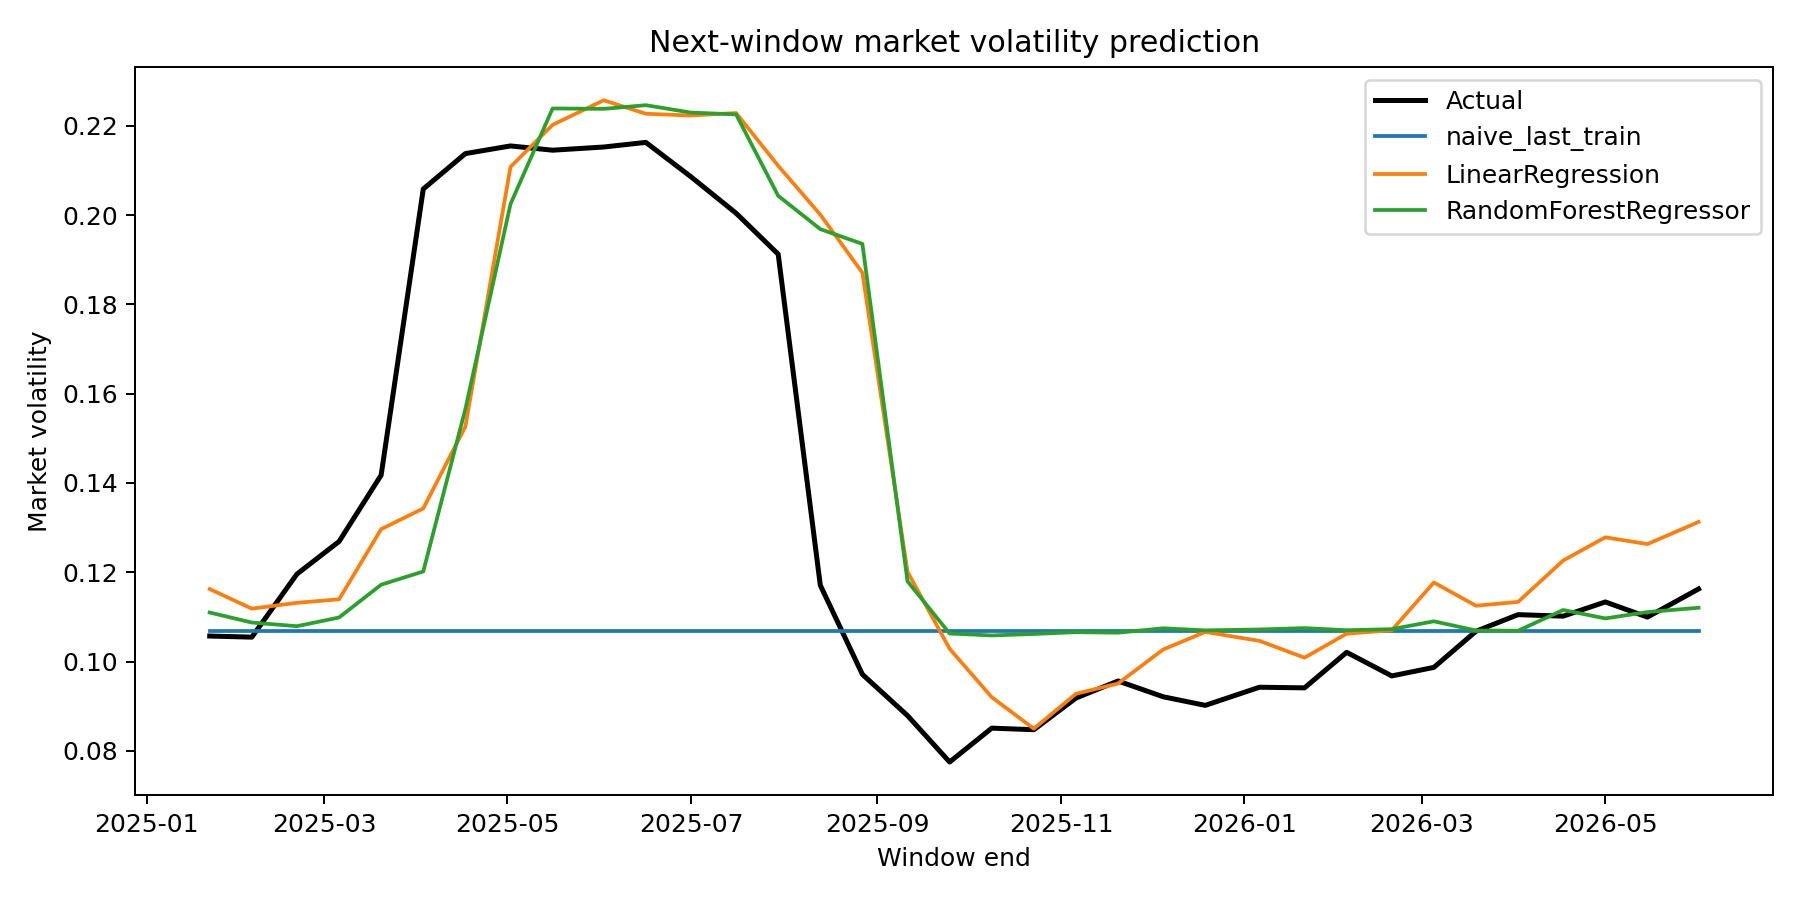
\includegraphics[width=0.86\textwidth]{../outputs/figures/prediction_comparison.png}
\caption{下一窗口市场波动率预测对比}
\label{fig:prediction}
\end{figure}

\section{对齐诊断与稳健性}
坐标对齐的目标是让动画稳定，而不是改变结构尺度。修复后的对齐诊断显示，最后窗口原始坐标范数为0.888，对齐坐标范数也为0.888；原始平均两两距离为1.159，对齐平均两两距离为1.159，距离比为1.000。所有窗口的距离比最小值为1.000，最大值为1.000。该结果表明，Procrustes对齐仅执行平移、旋转和镜像，没有引入递归缩放。由此，最新市场结构图中的坐标不再坍缩到机器精度，动画中股票位置变化反映的是MDS结构变化，而非数值误差。

数据质量方面，最终样本没有无效价格、重复记录或单日绝对对数收益超过0.5的异常记录。覆盖率筛选后46只股票全部保留。价格复权状态仍为unknown，这是本研究的重要限制：如果\texttt{close}并非复权价格，长期收益率中可能包含拆股、分红或其他公司行为影响。本文通过异常收益检测降低明显跳变的风险，但没有自行猜测拆股比例，也没有改写原始价格。

\section{局限性}
第一，数据来源只能判断为Stooq-style，未被独立说明文件确认。第二，价格字段缺少adjusted close，复权状态为unknown，因此不能把价格称为已复权价格。第三，股票池固定为46只大市值股票，代表性强于小样本个股研究，但不能覆盖完整美国市场。第四，MDS二维嵌入会损失高维距离信息，图形应被理解为相关结构的近似展示。第五，聚类数固定为6，便于跨窗口比较，但不同窗口的最佳聚类数可能不同。第六，预测实验窗口数有限，且仅使用窗口级滞后特征，因此结论不应扩展为投资建议。

\section{结论}
本文基于真实日频股票数据，构建了一个从数据检查、清洗、滚动窗口建模、相关距离、MDS、聚类、Procrustes对齐到预测实验的完整数据挖掘流程。实证结果显示，近五年美国大市值股票市场结构并不稳定：在2022年中后期，平均相关性、市场波动率和PC1解释率同步上升，二维结构更加集中；到最新窗口，平均相关性和共同因子强度明显下降，股票间二维距离扩大，市场结构更分散。行业标签与数据驱动聚类之间存在中等程度联系，但聚类编号不能直接解释为行业。简单预测实验显示，滞后结构指标能在测试集上优于naive baseline，但该结果仅说明窗口指标具有短期统计延续性，不构成投资建议。

\section*{免责声明}
本分析仅为数据挖掘课程实验，不构成投资建议。

\begin{thebibliography}{99}
\bibitem{Mantegna1999}
Mantegna, R. N. (1999). Hierarchical structure in financial markets. \textit{The European Physical Journal B}, 11, 193-197.

\bibitem{Torgerson1952}
Torgerson, W. S. (1952). Multidimensional scaling: I. Theory and method. \textit{Psychometrika}, 17(4), 401-419.

\bibitem{Kruskal1964}
Kruskal, J. B. (1964). Multidimensional scaling by optimizing goodness of fit to a nonmetric hypothesis. \textit{Psychometrika}, 29(1), 1-27.

\bibitem{Jolliffe2002}
Jolliffe, I. T. (2002). \textit{Principal Component Analysis}. 2nd edition. Springer.

\bibitem{Schonemann1966}
Schonemann, P. H. (1966). A generalized solution of the orthogonal Procrustes problem. \textit{Psychometrika}, 31(1), 1-10.

\bibitem{HubertArabie1985}
Hubert, L., and Arabie, P. (1985). Comparing partitions. \textit{Journal of Classification}, 2, 193-218.

\bibitem{Hastie2009}
Hastie, T., Tibshirani, R., and Friedman, J. (2009). \textit{The Elements of Statistical Learning}. 2nd edition. Springer.

\bibitem{Pedregosa2011}
Pedregosa, F., Varoquaux, G., Gramfort, A., Michel, V., Thirion, B., Grisel, O., Blondel, M., Prettenhofer, P., Weiss, R., Dubourg, V., Vanderplas, J., Passos, A., Cournapeau, D., Brucher, M., Perrot, M., and Duchesnay, E. (2011). Scikit-learn: Machine learning in Python. \textit{Journal of Machine Learning Research}, 12, 2825-2830.
\end{thebibliography}

\end{document}
